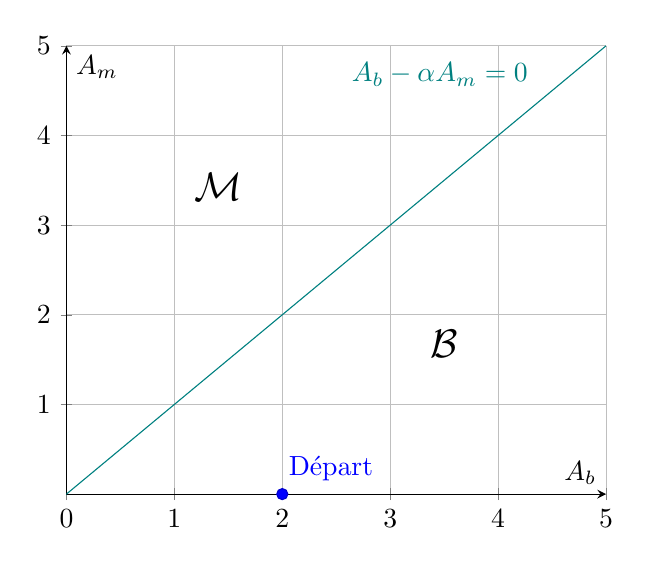
\begin{tikzpicture}
	\begin{axis}[
		grid=major,
		axis lines=middle,
		axis x line=bottom,  
		xlabel=$A_b$,
		ylabel=$A_m$,
		xmin=0,xmax=5,
		ymin=0,ymax=5,
		% xtick={0,...,9},
	]

	\addplot[teal] {\x} node[midway,above]{ };

	\addplot[scatter, only marks, mark=*, mark size=2pt, teal] coordinates {
		(2,0)
	};
	\end{axis}


	\node[anchor=north west, teal] at (3.5, 5.6) {$A_b - \alpha A_m = 0$};
	\node[anchor=north west, blue] at (2.7,0.6) {Départ};
	\node[anchor=north west] at (1.5,4.2) {\Large $\mathcal{M}$};
	\node[anchor=north west] at (4.5,2.2) {\Large $\mathcal{B}$};
\end{tikzpicture}